\subsection{Gradiente Normalizado}

Nas simula��es, procuramos avaliar o comportamento do sistema para as seguintes condi��es:
%
\begin{enumerate*}[label=(\roman*)]
\item condi��o inicial $\theta(0)$;
\item sinal de refer�ncia $r(t)$;
\item ganho de adapta��o $\gamma$.
\end{enumerate*}

Apresentaremos os resultados obtidos atrav�s de simula��es no ambiente \HI{\texttt{Matlab/Simulink}} e os discutiremos na pr�xima se��o.

\subsection{Simula��o \#1}

Inicialmente, desejamos verificar o comportamento do sistema para varia��es no
sinal de refer�ncia $r(t)$ para podermos analisar a influ�ncia da persist�ncia
de excita��o.

%\bigskip%
%Par�metros e condi��es iniciais :
%
\begin{align*}
  y &= \frac{1}{s+2}u\,,  &  \Lambda &= \frac{1}{s+1}\,, & \theta(0) &= 0\,, \\
  \gamma &= 5\,, & r &= \HI{1, $1+5\textrm{sin}(t)$}\, \,.
\end{align*}

\bigskip%
\begin{figure}[H]
  \centering
  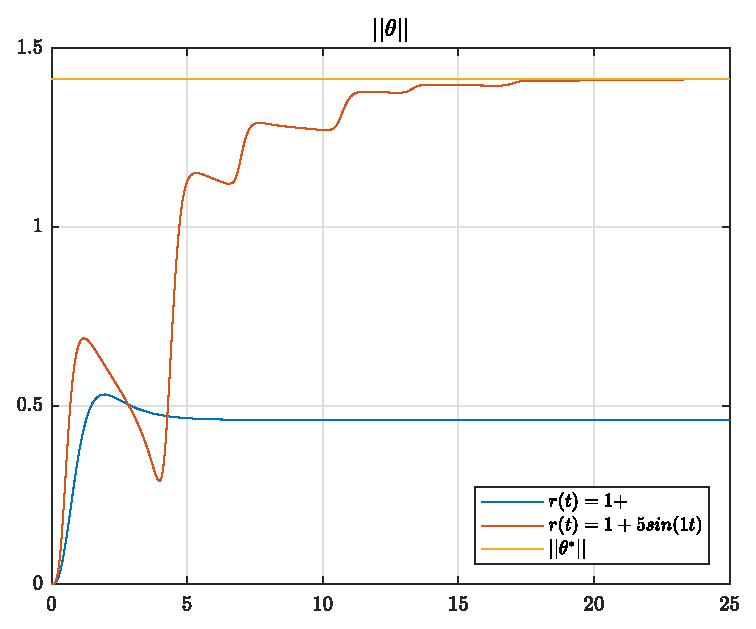
\includegraphics[width=12cm]{figs/gradiente/modtheta/sim01_r1r2.eps} \\[2mm]
\end{figure}

\begin{figure}[H]
  \centering
  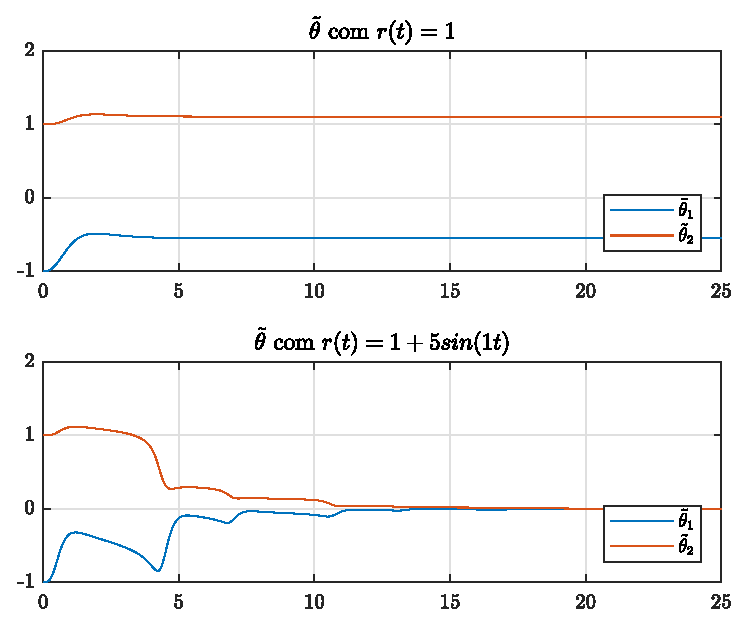
\includegraphics[width=12cm]{figs/gradiente/tiltheta/sim01_r1r2.eps} 
\end{figure}


\begin{figure}[H]
  \centering
  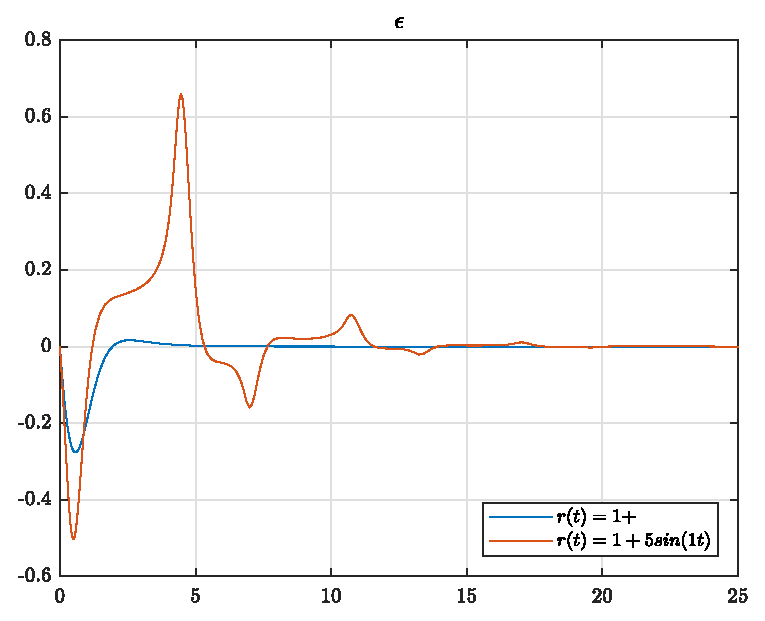
\includegraphics[width=12cm]{figs/gradiente/epsilon/sim01_r1r2.eps} 
\end{figure}

\newpage%

\begin{align*}
  y &= \frac{s+1}{s+4s+4}u\,,  &  \Lambda &= \frac{1}{s^2+2s+1}\,, & \theta(0)
  &= 0\,,\\
  \gamma &= 10\,, & r &= \HI{$10\textrm{sin}(0.63493t)$} e
  \HI{$30\textrm{sin}(0.63493t)+25\textrm{sin}(4.5669t)$}\, \,.
\end{align*}

\bigskip%
\begin{figure}[H]
  \centering
  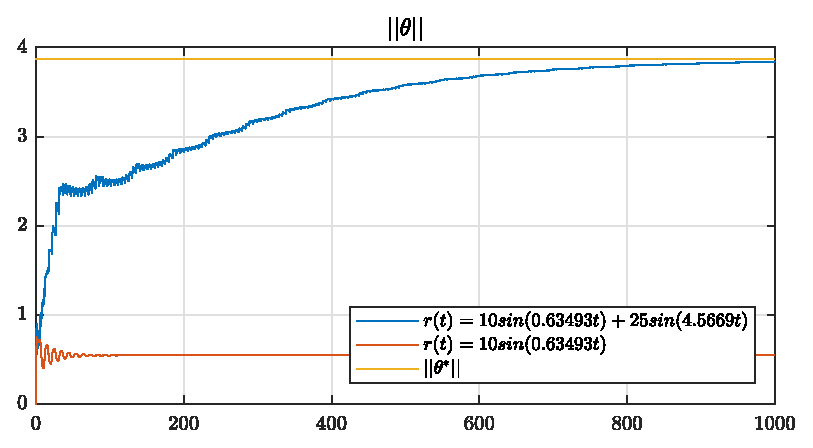
\includegraphics[width=12cm]{figs/gradiente/modtheta/sim02_r1r2.eps} \\[2mm]
\end{figure}

\begin{figure}[H]
  \centering
  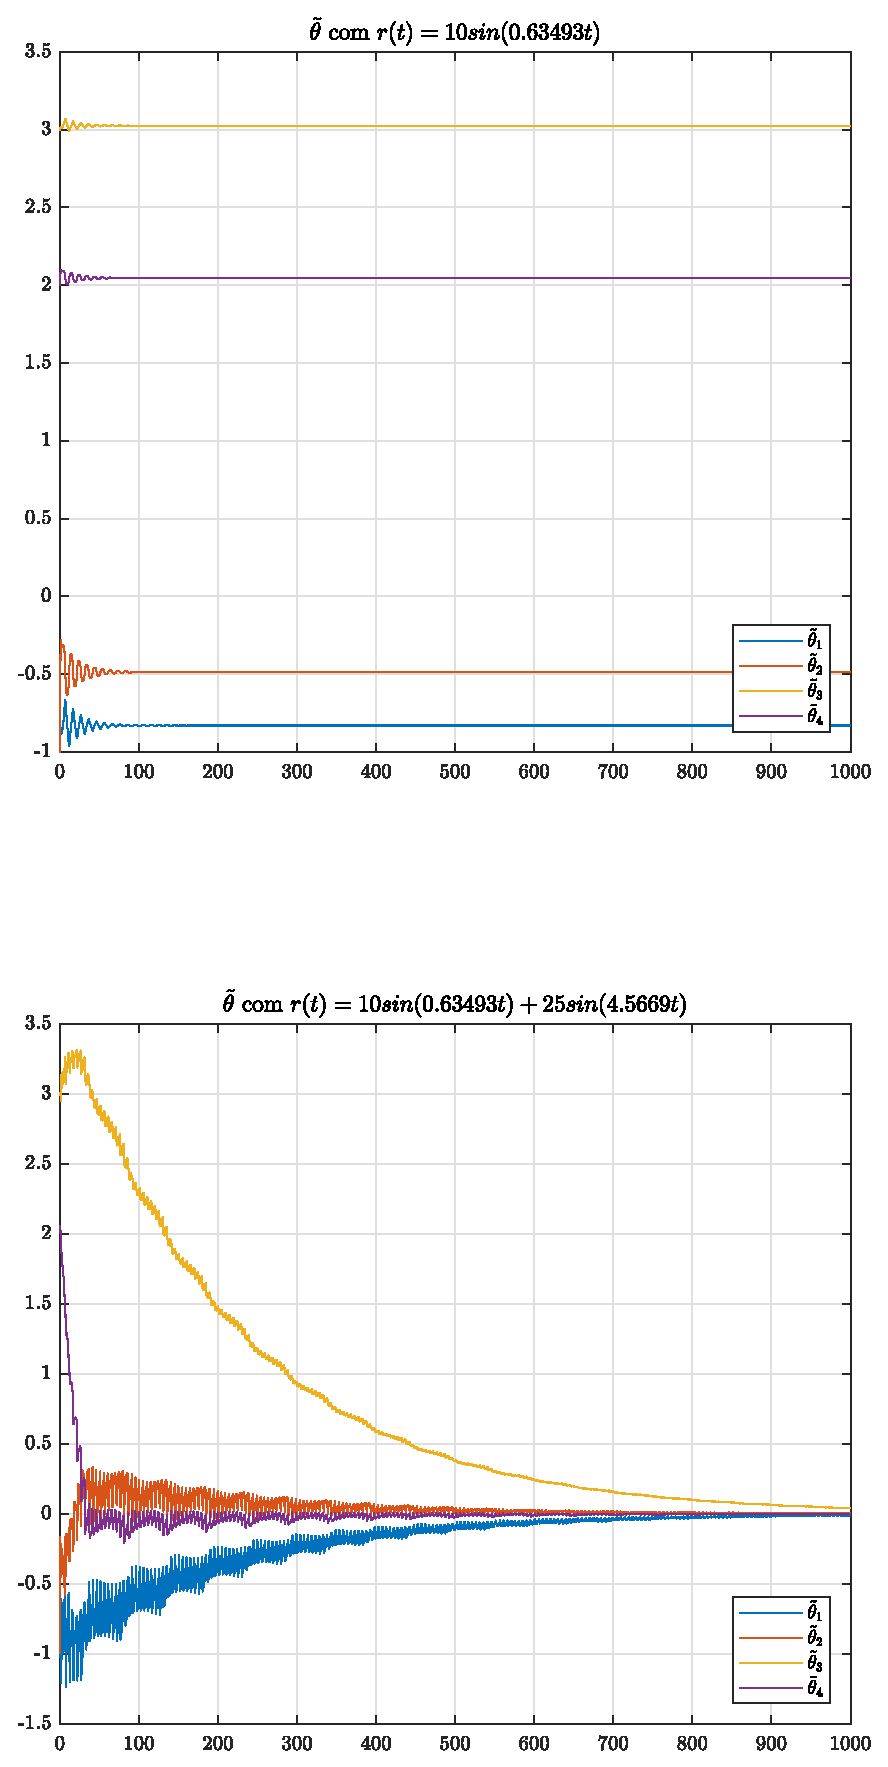
\includegraphics[width=12cm]{figs/gradiente/tiltheta/sim02_r1r2.eps} 
\end{figure}


\begin{figure}[H]
  \centering
  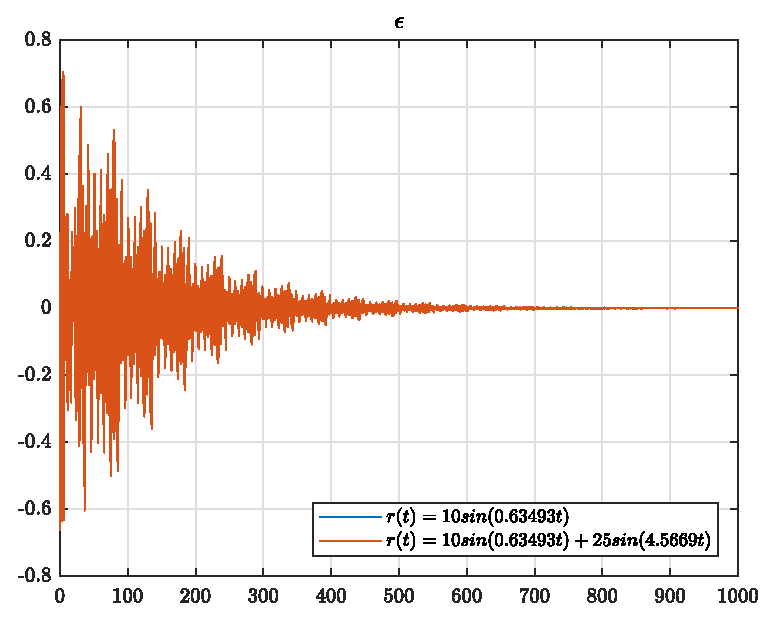
\includegraphics[width=12cm]{figs/gradiente/epsilon/sim02_r1r2.eps} 
\end{figure}

\newpage%

\begin{align*}
  y &= \frac{s+2s+1}{s^2+6s^2+12s+8}u\,,  &  \Lambda &=
  \frac{1}{s^3+3s^2+3s+1}\,, & \theta(0) &= 0\,,\\
  \gamma &= 10\,, & r &= \, \,.
\end{align*}

\bigskip%
\begin{figure}[H]
  \centering
  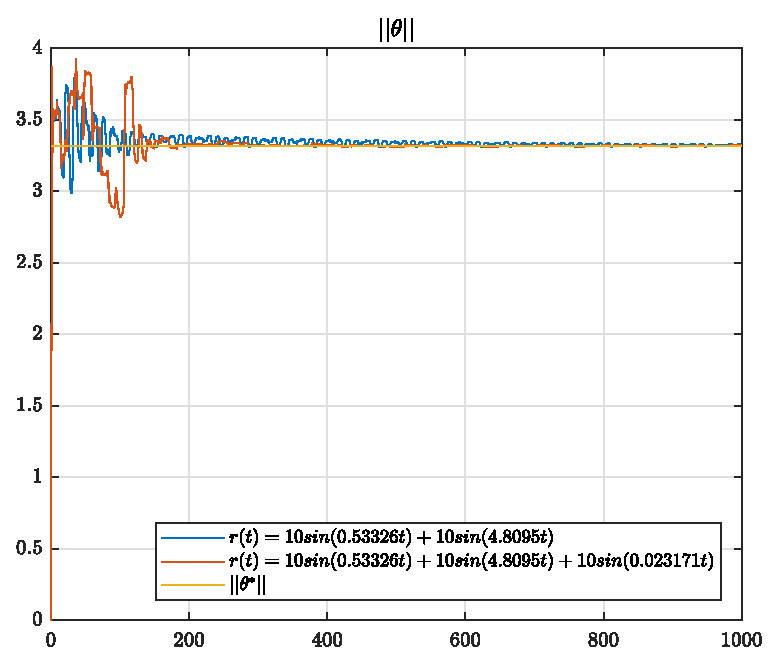
\includegraphics[width=12cm]{figs/gradiente/modtheta/sim03_r1r2.eps} \\[2mm]
\end{figure}

\begin{figure}[H]
  \centering
  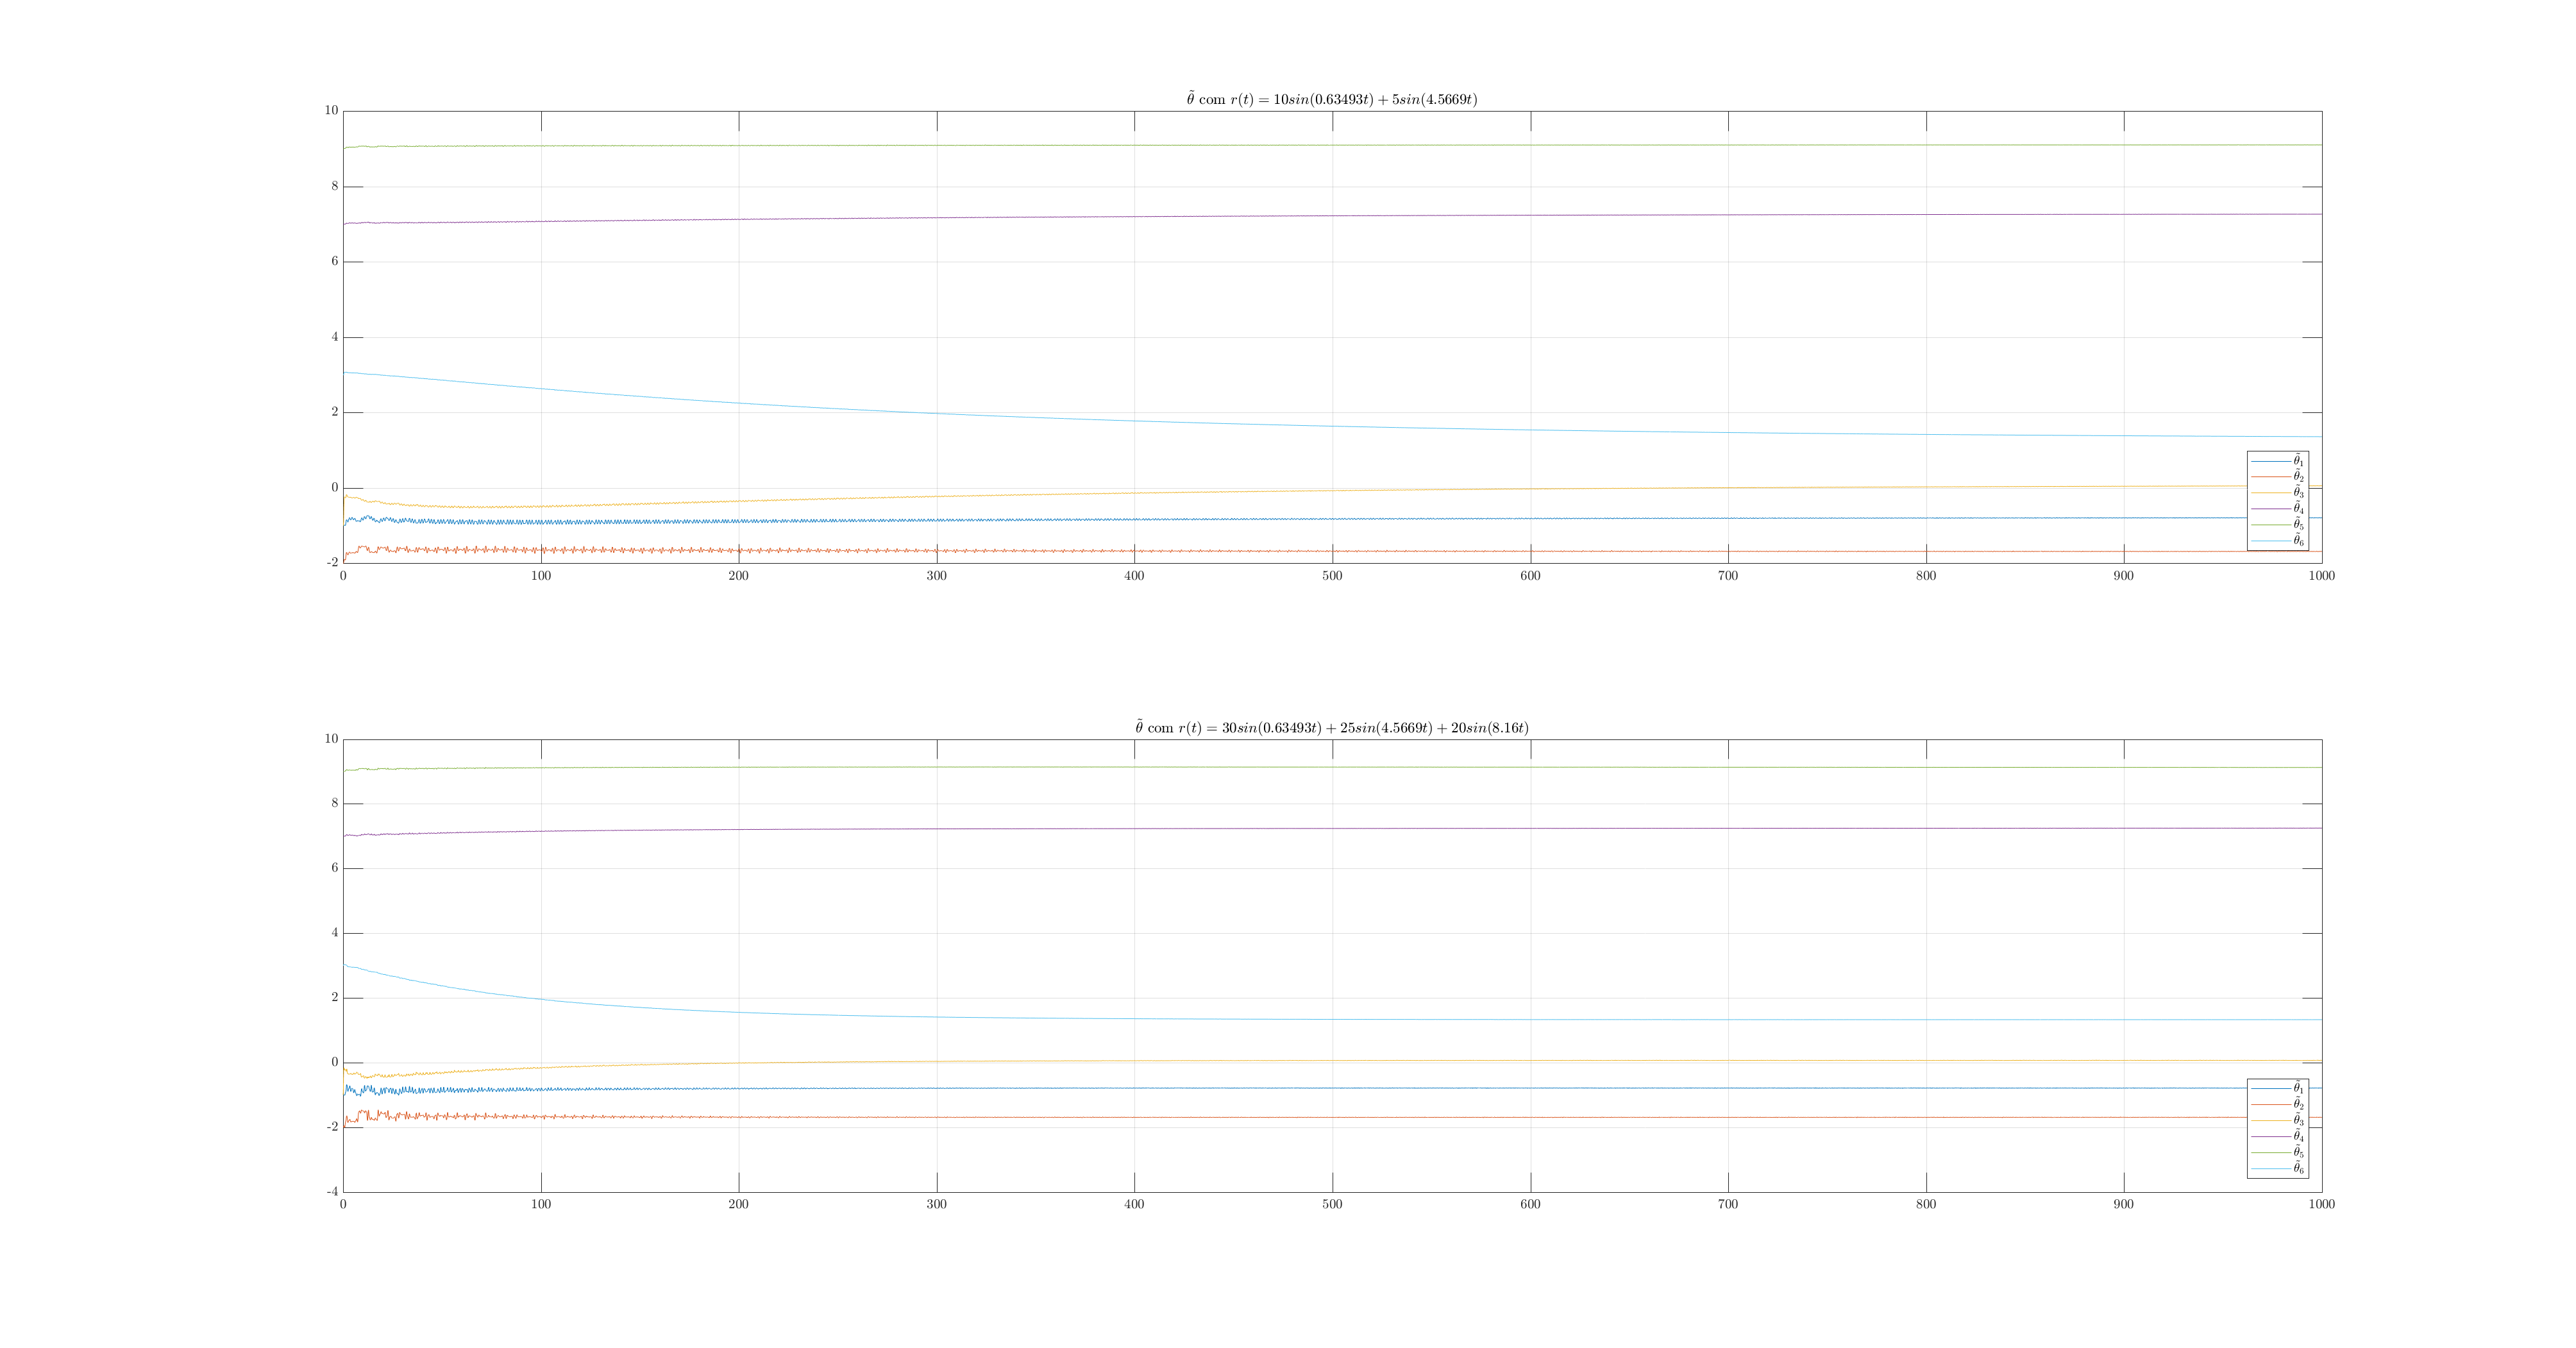
\includegraphics[width=12cm]{figs/gradiente/tiltheta/sim03_r1r2.eps} 
\end{figure}


\begin{figure}[H]
  \centering
  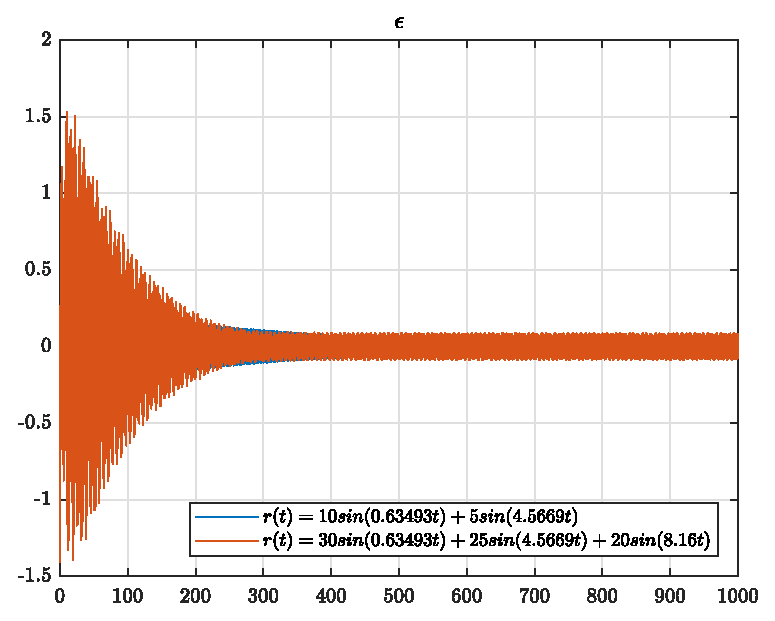
\includegraphics[width=12cm]{figs/gradiente/epsilon/sim03_r1r2.eps} 
\end{figure}
%---------------------------------------------------------------------
\subsection{Simula��o \#2}

Na segunda simula��o, observamos o comportamento do sistema para varia��es no
ganho de adapta��o.

\begin{align*}
  y &= \frac{1}{s+2}u\,,  &  \Lambda &= \frac{1}{s+1}\,, & \theta(0) &= 0\,, \\
  \gamma &= \HI{5, 10}\,, & r &= 1+5\textrm{sin}(t)\, \,.
\end{align*}

\bigskip%
\begin{figure}[H]
  \centering
  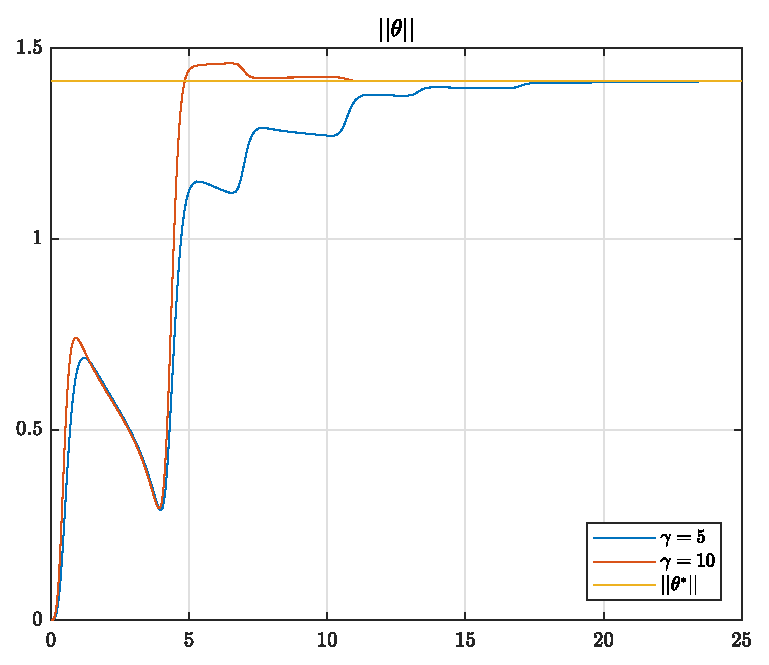
\includegraphics[width=12cm]{figs/gradiente/modtheta/sim01_gamma5gamma10.eps} \\[2mm]
\end{figure}

\begin{figure}[H]
  \centering
  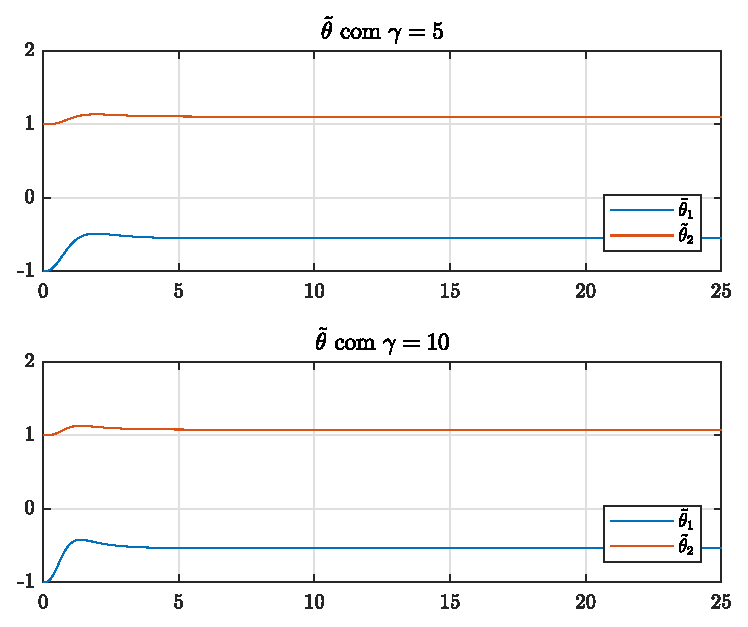
\includegraphics[width=12cm]{figs/gradiente/tiltheta/sim01_gamma5gamma10.eps} 
\end{figure}


\begin{figure}[H]
  \centering
  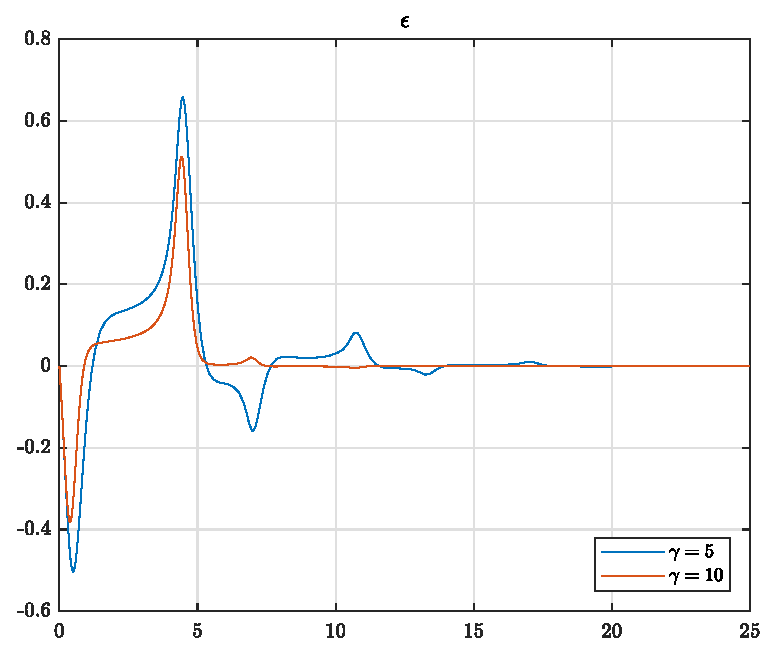
\includegraphics[width=12cm]{figs/gradiente/epsilon/sim01_gamma5gamma10.eps} 
\end{figure}

\newpage%

\begin{align*}
  y &= \frac{s+1}{s+4s+4}u\,,  &  \Lambda &= \frac{1}{s^2+2s+1}\,, & \theta(0)
  &= 0\,,\\
  \gamma &= \HI{1,10}\,, & r &=
  30\textrm{sin}(0.63493t)+25\textrm{sin}(4.5669t) \,.
\end{align*}

\bigskip%
\begin{figure}[H]
  \centering
  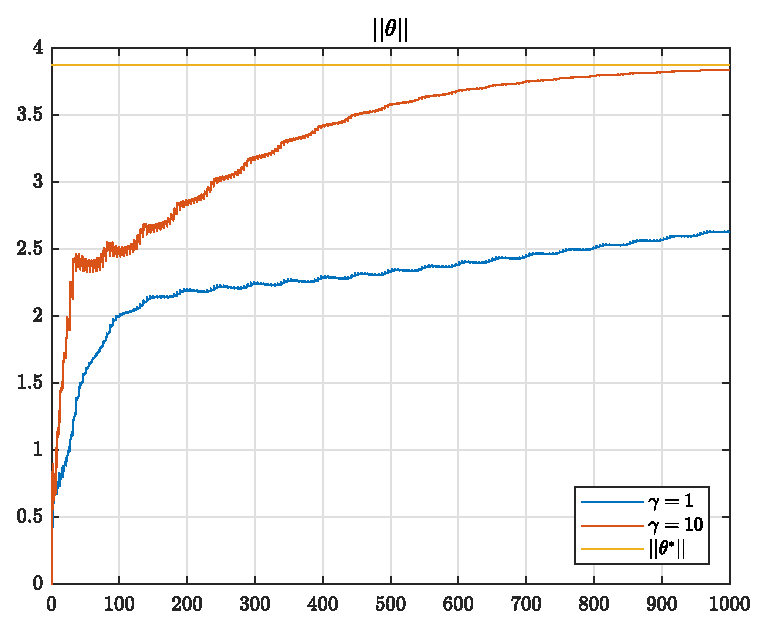
\includegraphics[width=12cm]{figs/gradiente/modtheta/sim02_gamma1gamma10.eps}
  \\[2mm]
\end{figure}

\begin{figure}[H]
  \centering
  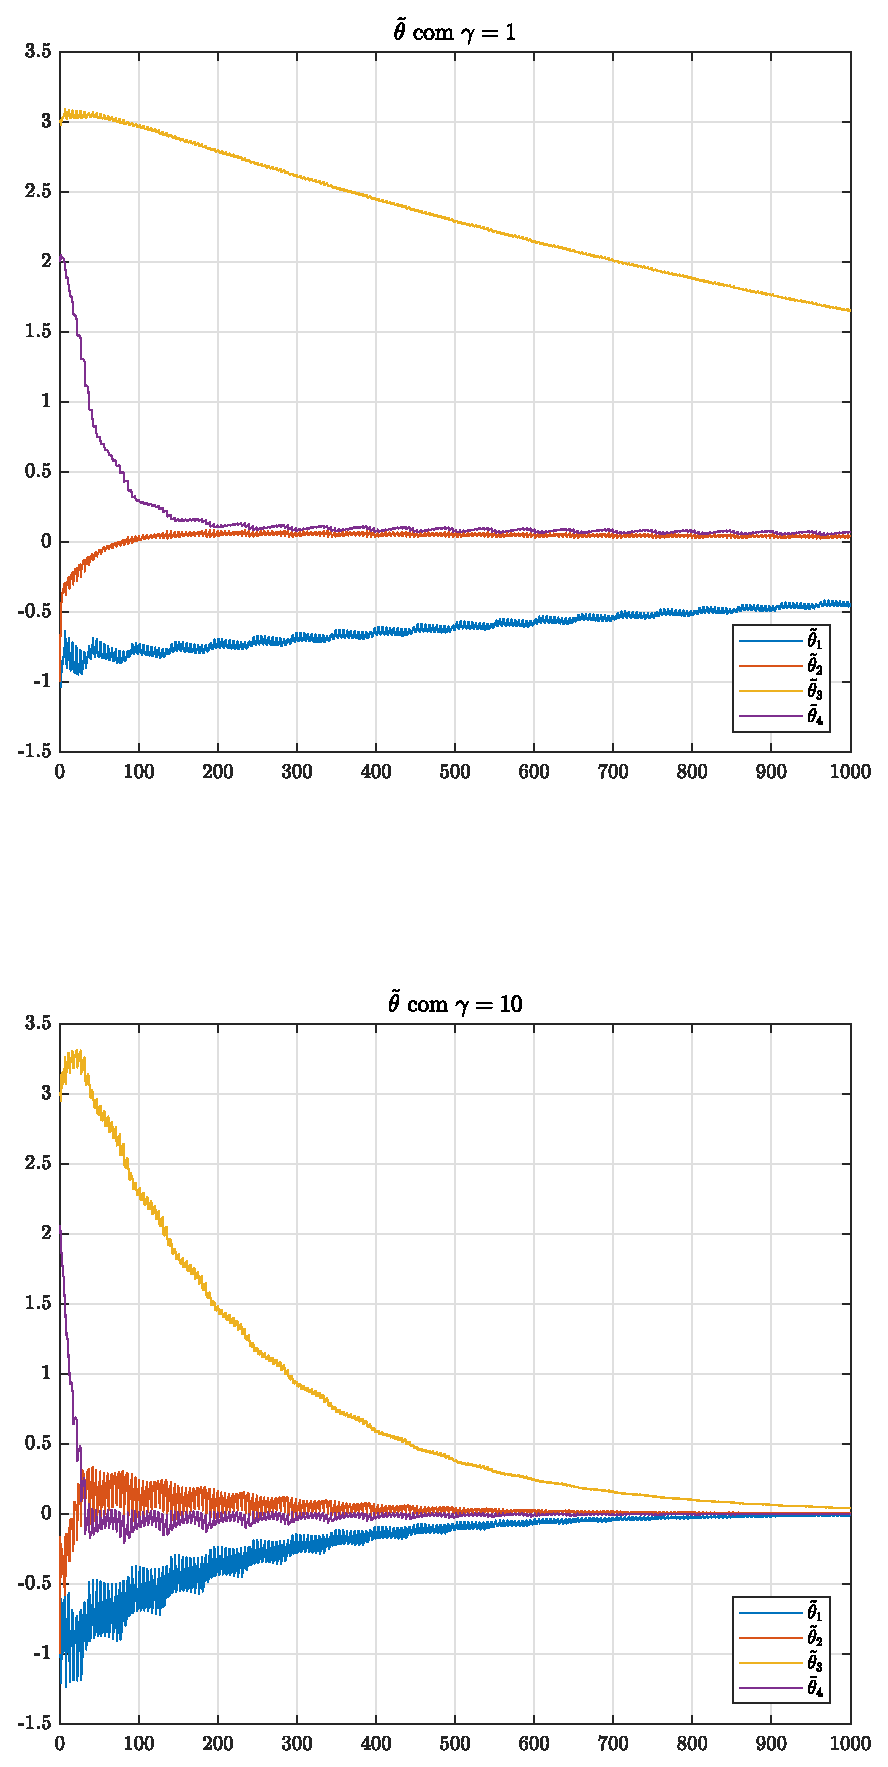
\includegraphics[width=12cm]{figs/gradiente/tiltheta/sim02_gamma1gamma10.eps} 
\end{figure}


\begin{figure}[H]
  \centering
  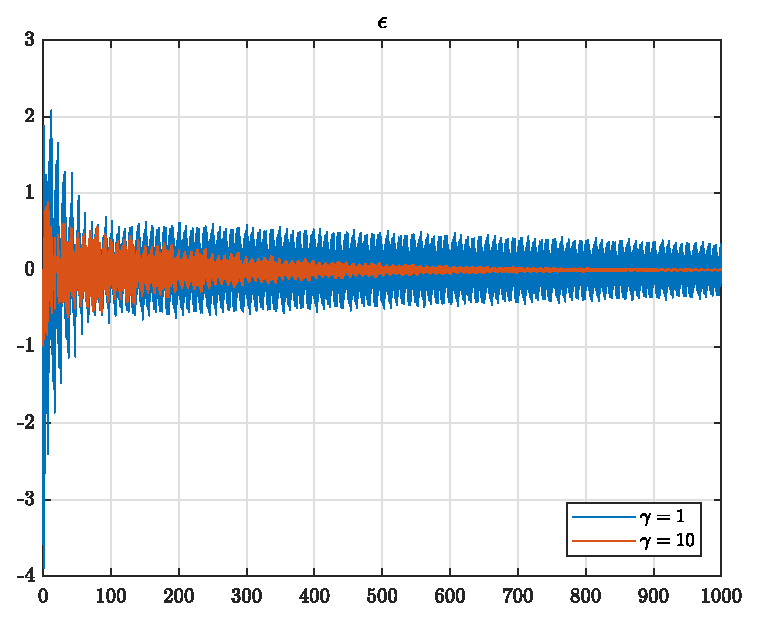
\includegraphics[width=12cm]{figs/gradiente/epsilon/sim02_gamma1gamma10.eps} 
\end{figure}

\newpage%

\begin{align*}
  y &= \frac{s+2s+1}{s^2+6s^2+12s+8}u\,,  &  \Lambda &=
  \frac{1}{s^3+3s^2+3s+1}\,, & \theta(0) &= 0\,,\\
  \gamma &= 10\,, & r &=  \,.
\end{align*}

\bigskip%
\begin{figure}[H]
  \centering
  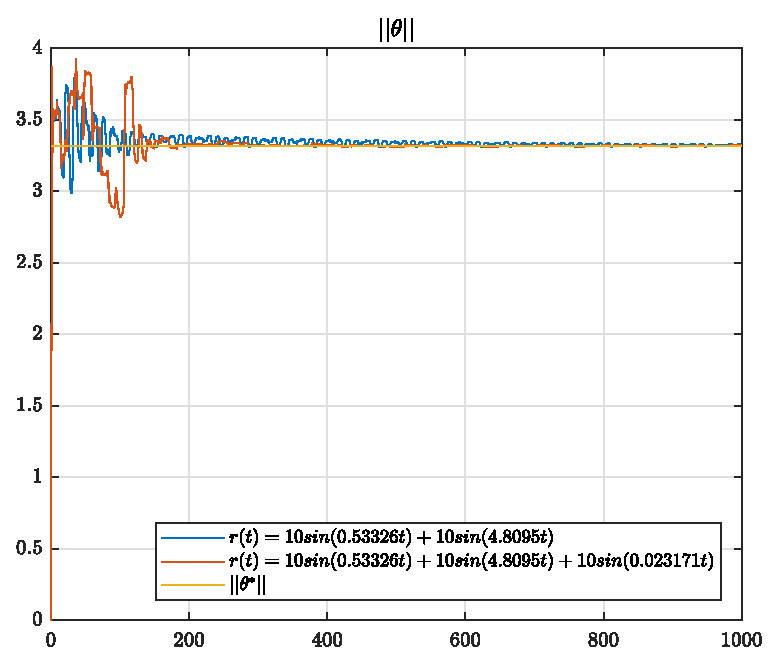
\includegraphics[width=12cm]{figs/gradiente/modtheta/sim03_r1r2.eps} \\[2mm]
\end{figure}

\begin{figure}[H]
  \centering
  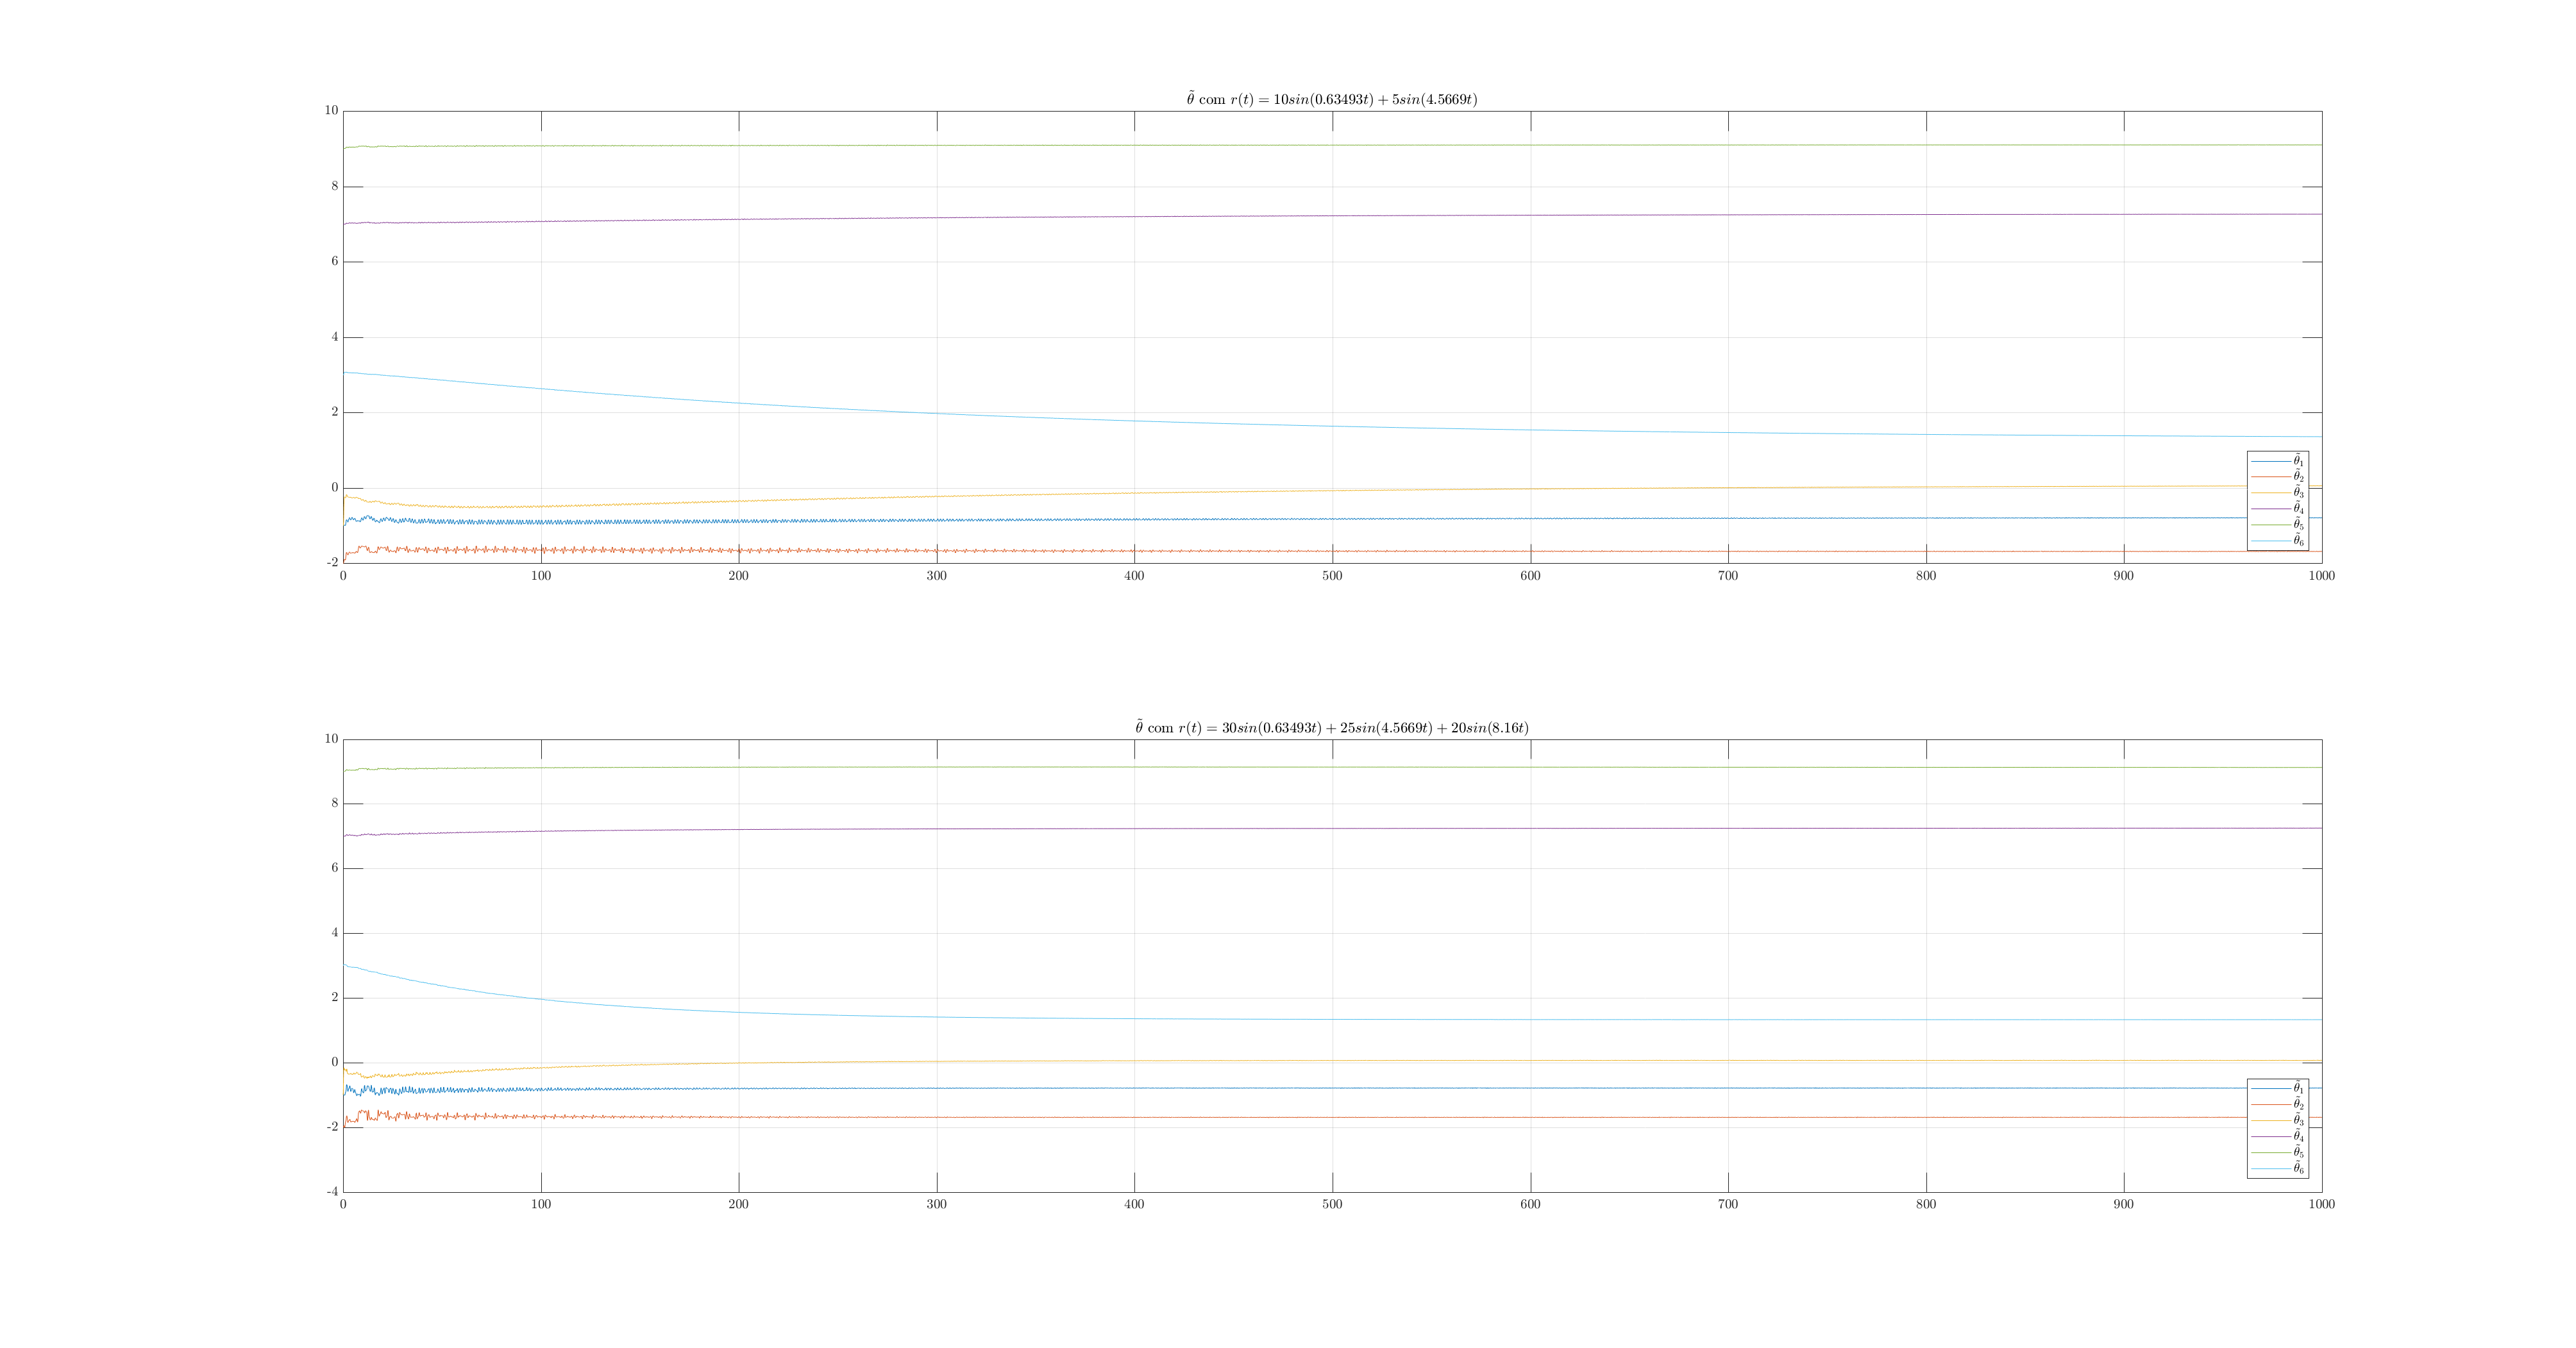
\includegraphics[width=12cm]{figs/gradiente/tiltheta/sim03_r1r2.eps} 
\end{figure}


\begin{figure}[H]
  \centering
  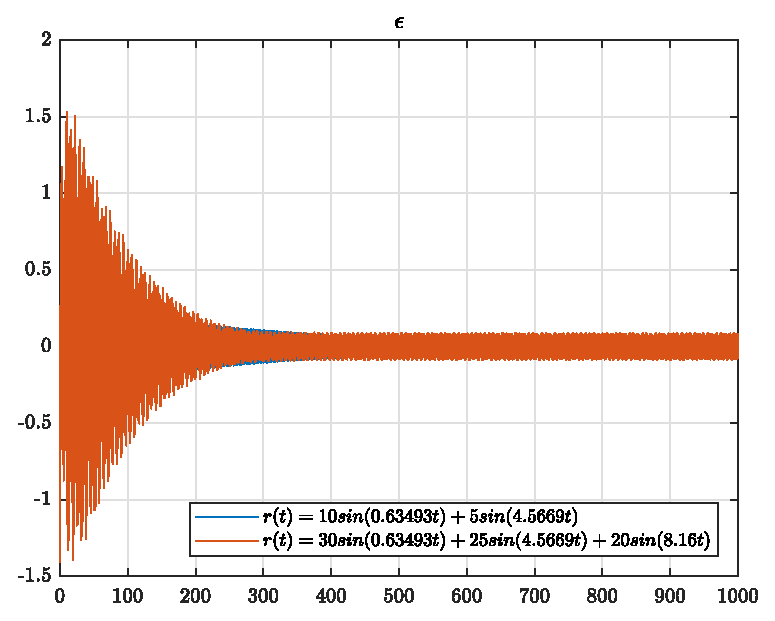
\includegraphics[width=12cm]{figs/gradiente/epsilon/sim03_r1r2.eps} 
\end{figure}
%---------------------------------------------------------------------
\subsection{Simula��o \#3}

Na terceira simula��o, observamos o comportamento do sistema para varia��es nas
condi��es iniciais do par�metro de estim��o $\theta$.

\begin{align*}
  y &= \frac{1}{s+2}u\,,  &  \Lambda &= \frac{1}{s+1}\,, & \theta(0) &= 0\,, \\
  \gamma &= 5\,, & r &= 1+5\textrm{sin}(t) \,.
\end{align*}

\bigskip%
\begin{figure}[H]
  \centering
  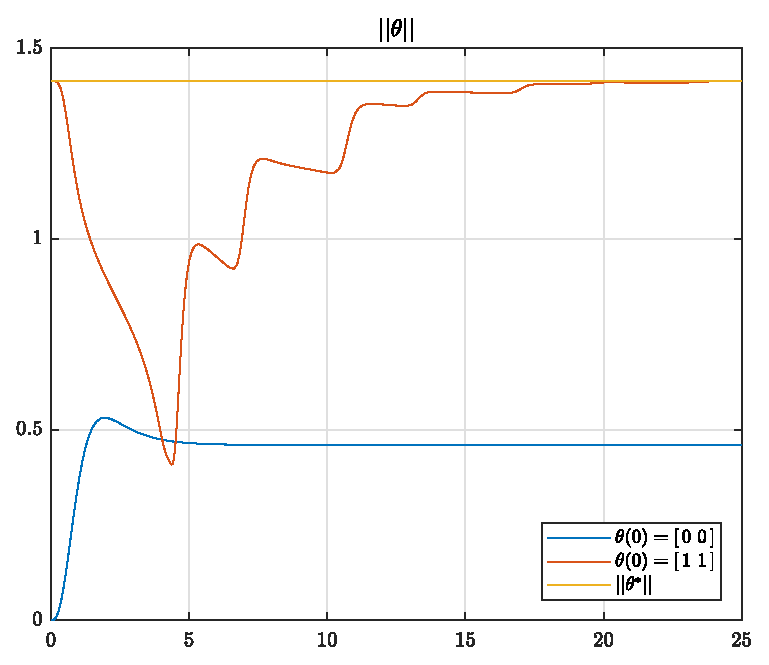
\includegraphics[width=12cm]{figs/gradiente/modtheta/sim01_theta01theta02.eps}
  \\[2mm]
\end{figure}

\begin{figure}[H]
  \centering
  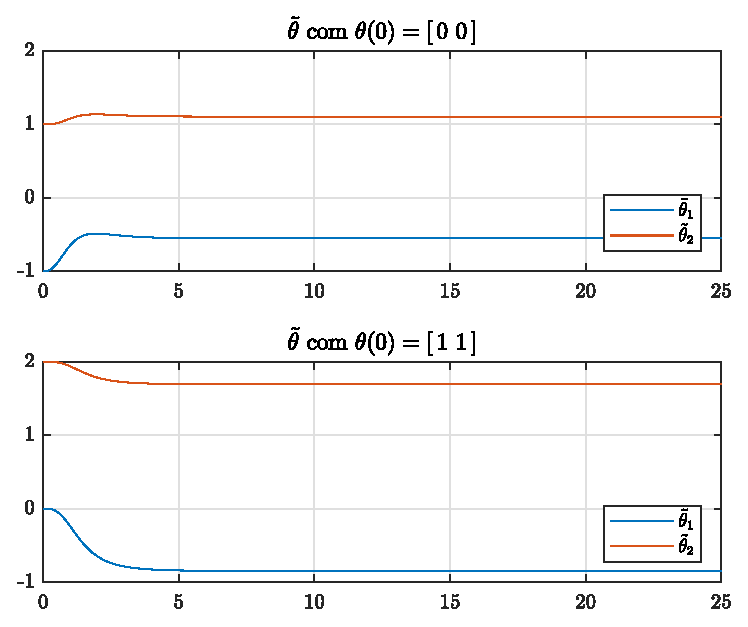
\includegraphics[width=12cm]{figs/gradiente/tiltheta/sim01_theta01theta02.eps} 
\end{figure}


\begin{figure}[H]
  \centering
  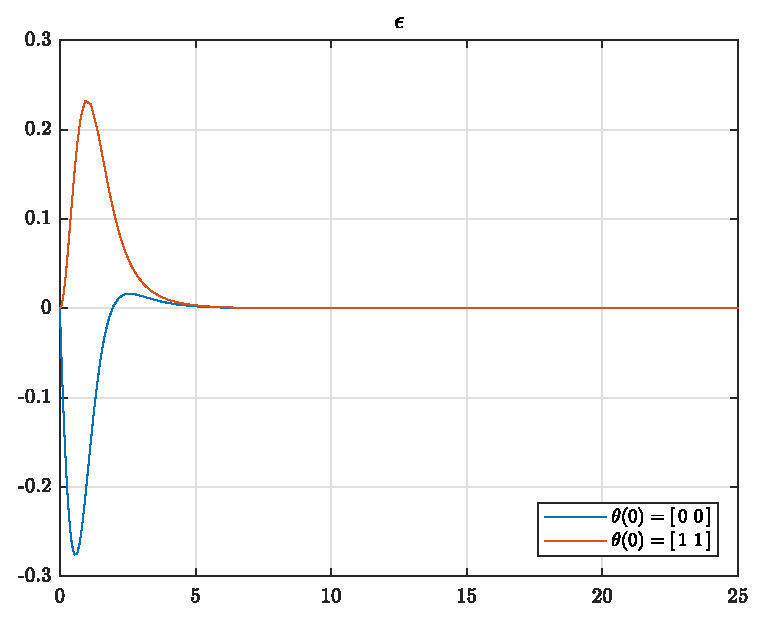
\includegraphics[width=12cm]{figs/gradiente/epsilon/sim01_theta01theta02.eps} 
\end{figure}

\newpage%

\begin{align*}
  y &= \frac{s+1}{s+4s+4}u\,,  &  \Lambda &= \frac{1}{s^2+2s+1}\,, & \theta(0)
  &= \HI{0, 1}\,,\\
  \gamma &= 10\,, & r &= 30\textrm{sin}(0.63493t)+25\textrm{sin}(4.5669t)\,.
\end{align*}

\bigskip%
\begin{figure}[H]
  \centering
  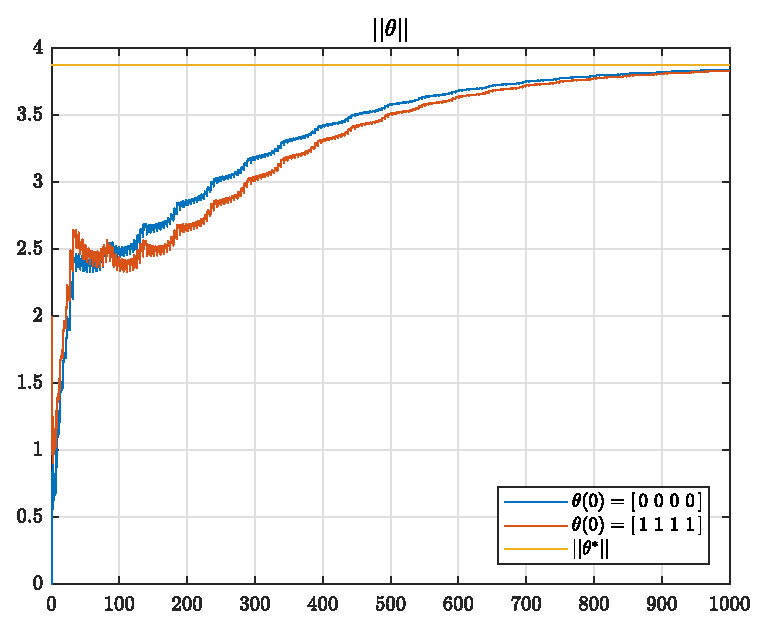
\includegraphics[width=12cm]{figs/gradiente/modtheta/sim02_theta01theta02.eps}
  \\[2mm]
\end{figure}

\begin{figure}[H]
  \centering
  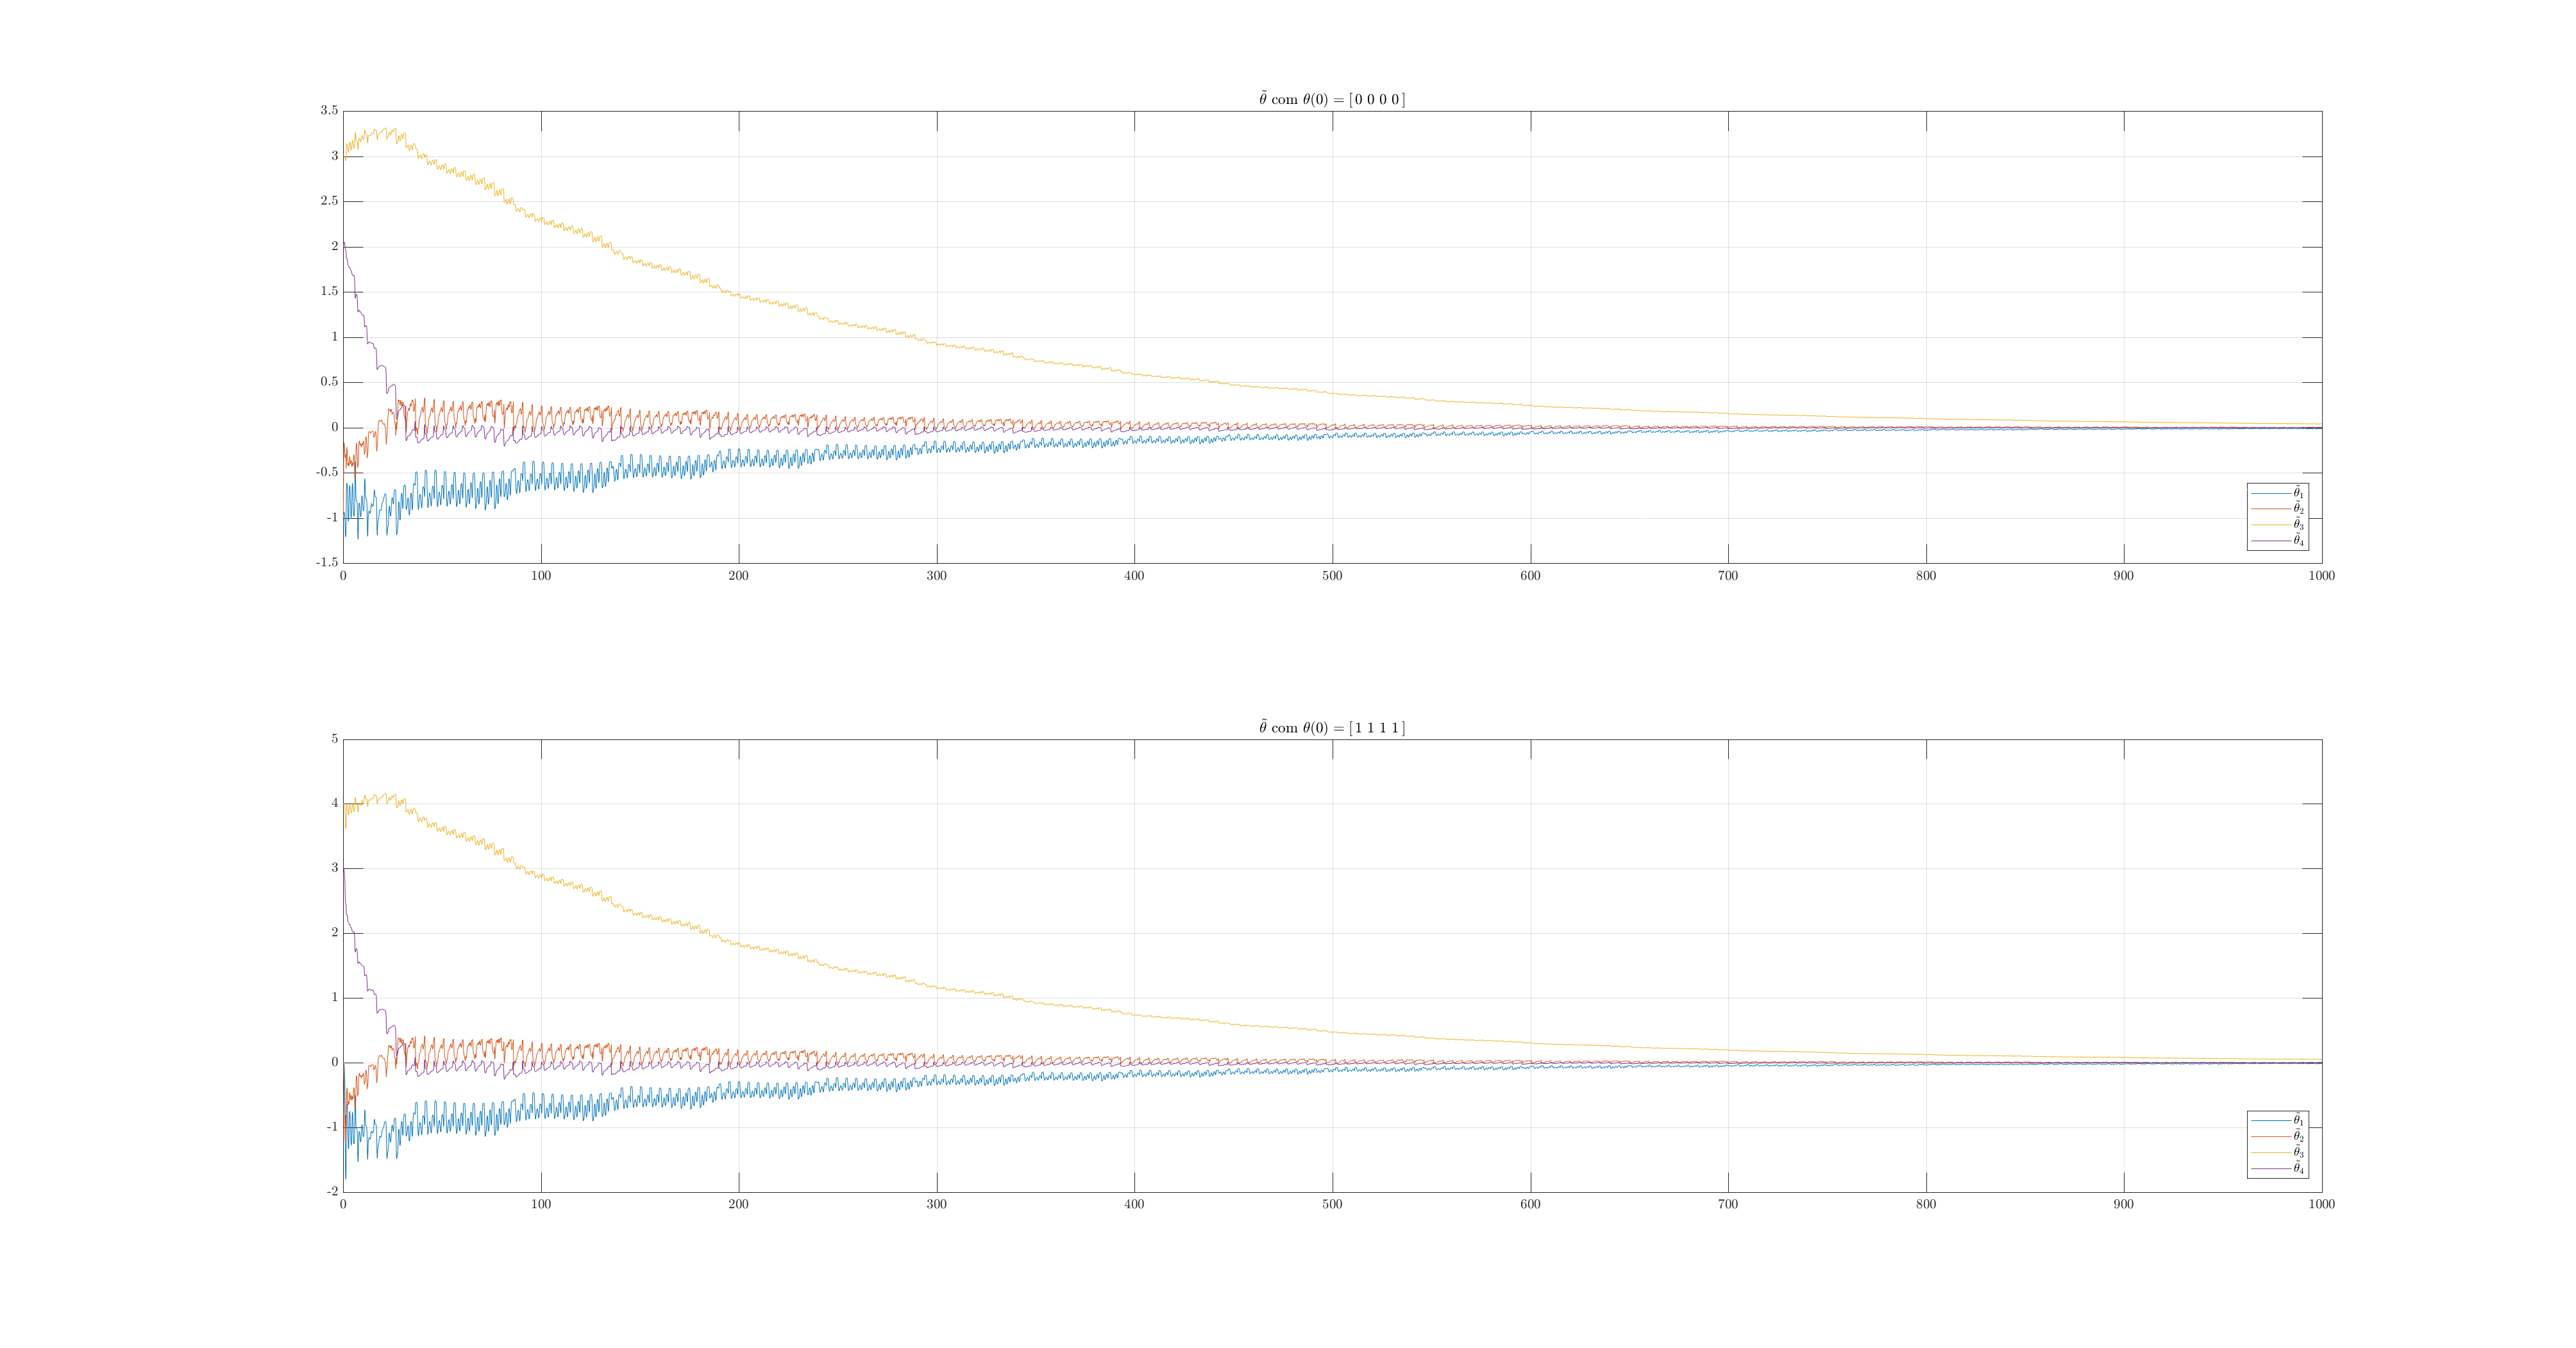
\includegraphics[width=12cm]{figs/gradiente/tiltheta/sim02_theta01theta02.eps} 
\end{figure}


\begin{figure}[H]
  \centering
  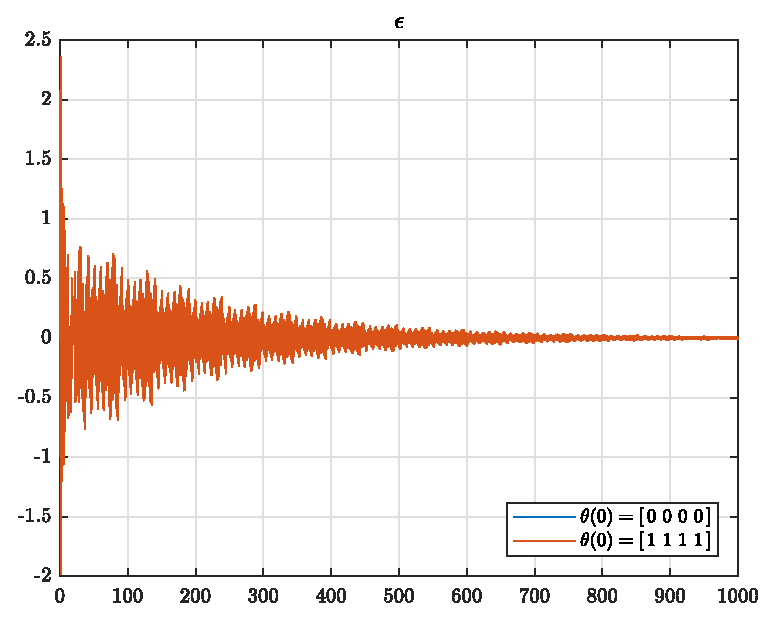
\includegraphics[width=12cm]{figs/gradiente/epsilon/sim02_theta01theta02.eps} 
\end{figure}

\newpage%

\begin{align*}
  y &= \frac{s+2s+1}{s^2+6s^2+12s+8}u\,,  &  \Lambda &=
  \frac{1}{s^3+3s^2+3s+1}\,, & \theta(0) &= 0\,,\\
  \gamma &= 10\,, & r &= \, \,.
\end{align*}

\bigskip%
\begin{figure}[H]
  \centering
  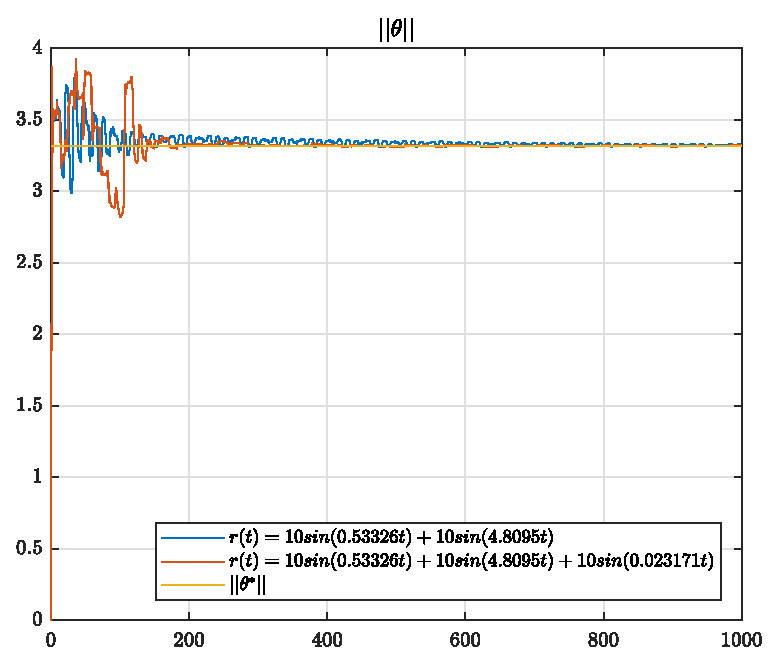
\includegraphics[width=12cm]{figs/gradiente/modtheta/sim03_r1r2.eps} \\[2mm]
\end{figure}

\begin{figure}[H]
  \centering
  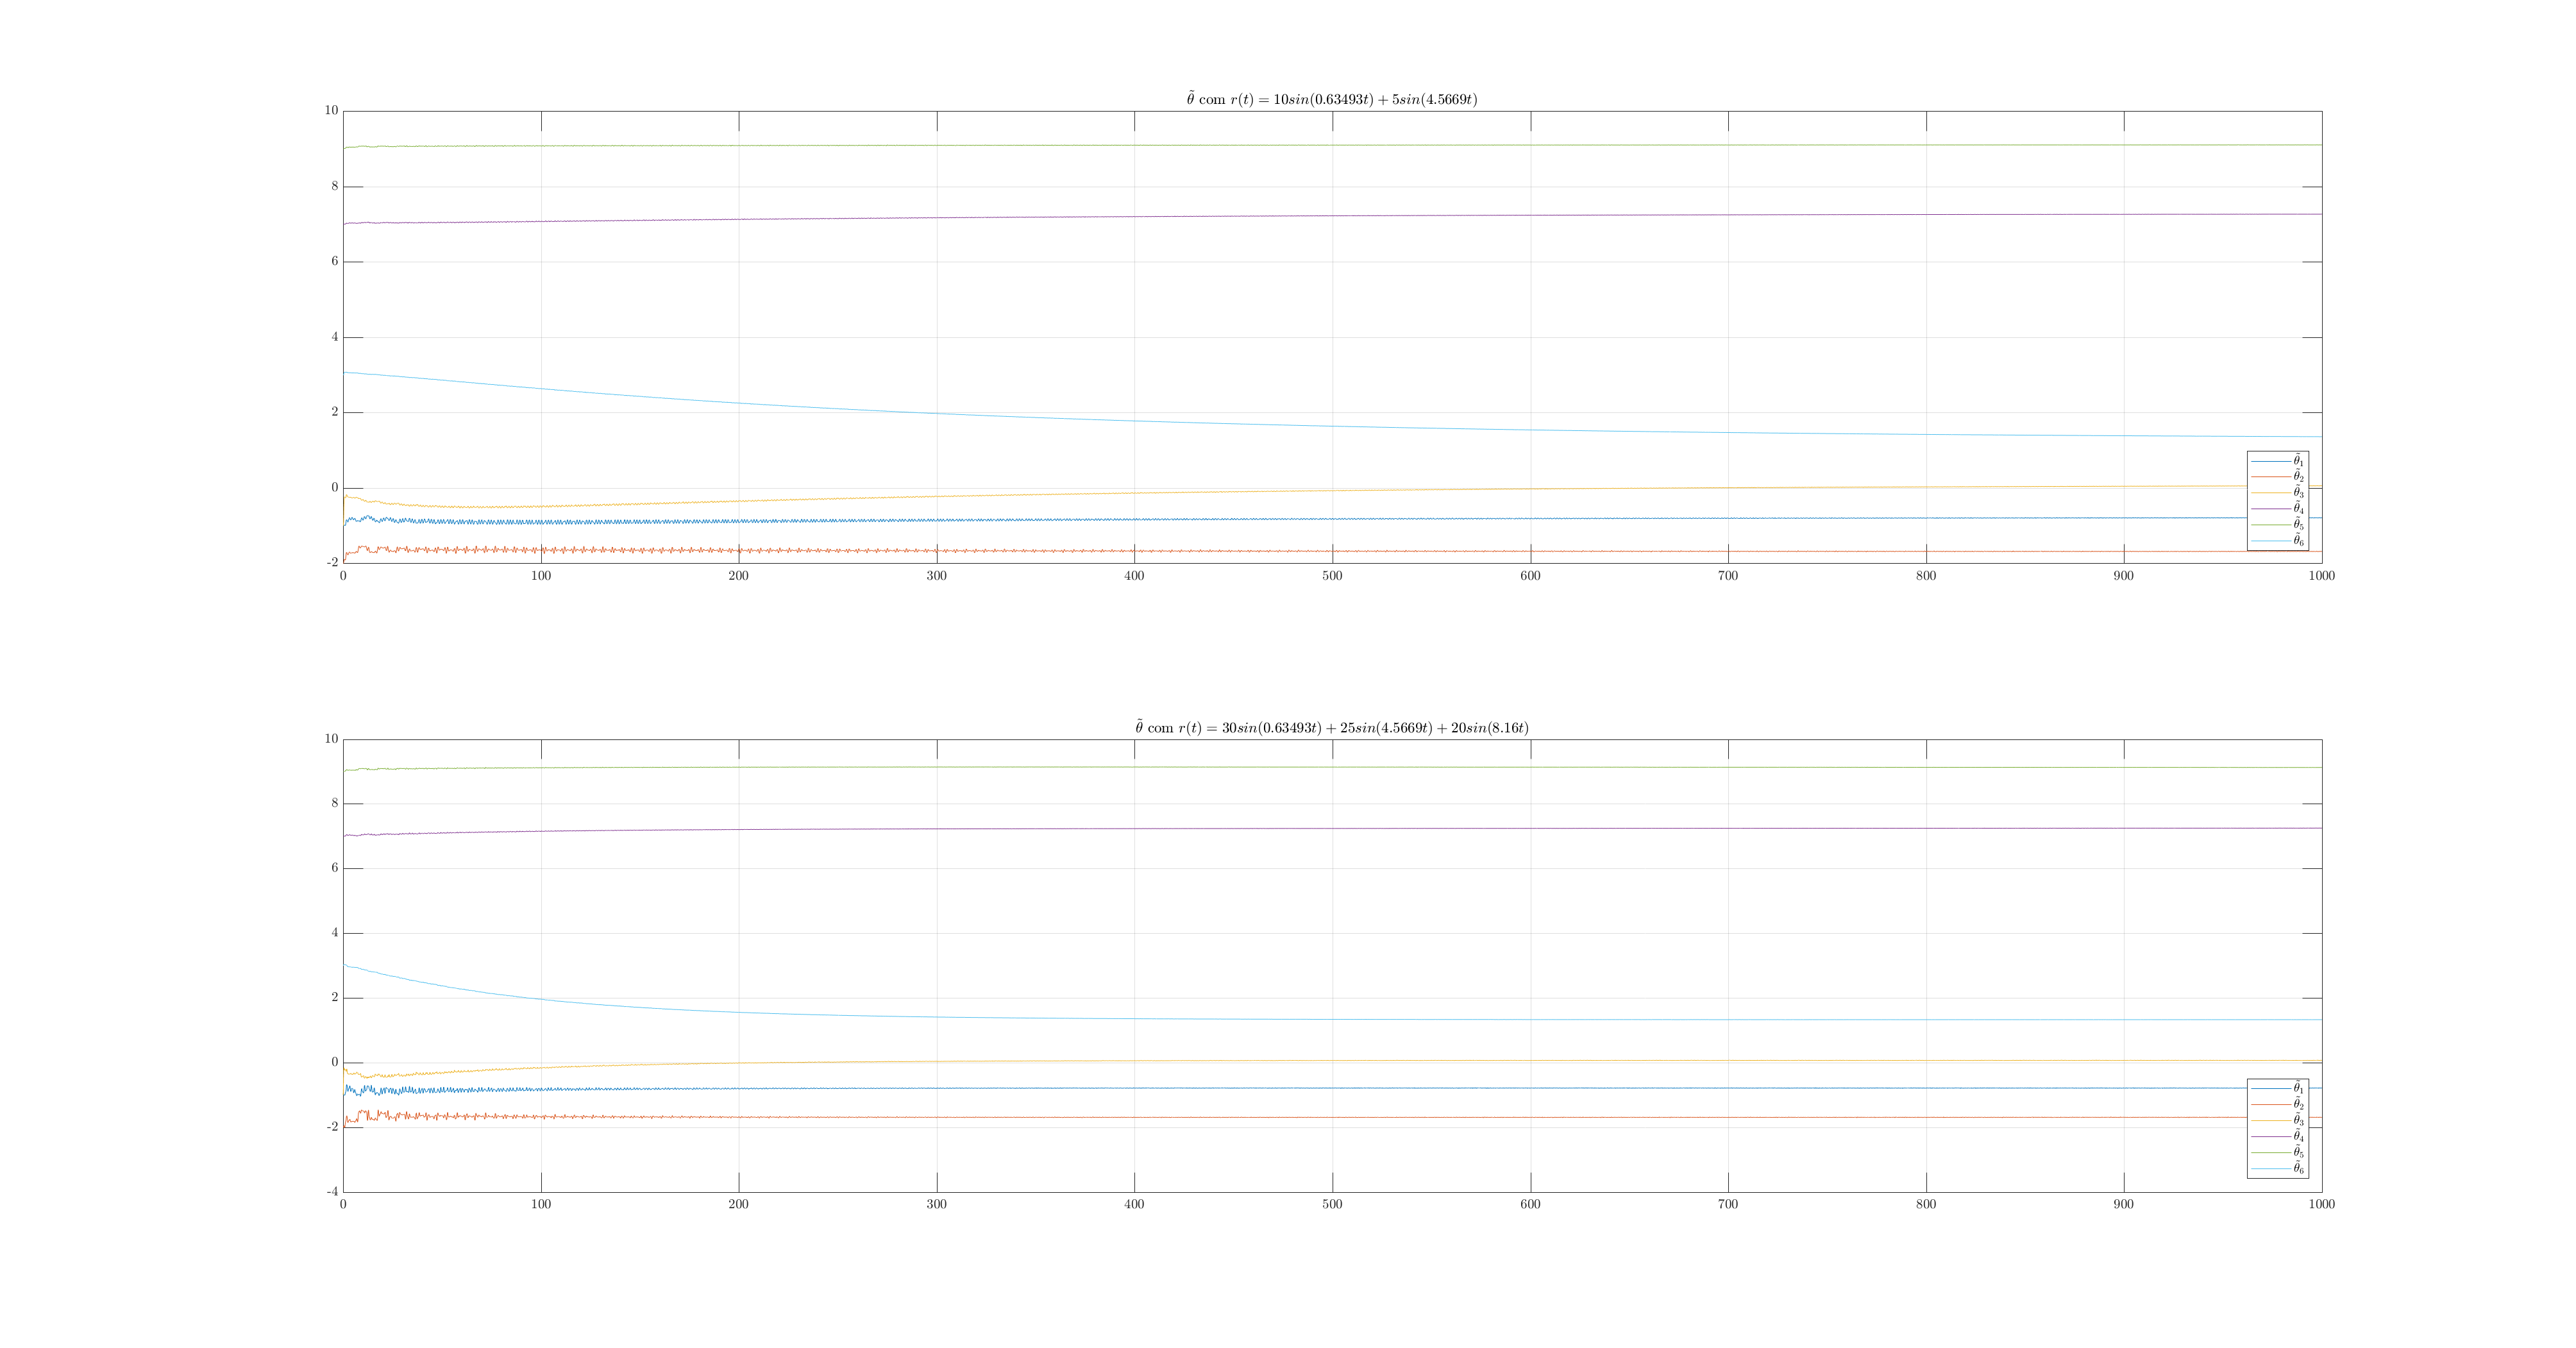
\includegraphics[width=12cm]{figs/gradiente/tiltheta/sim03_r1r2.eps} 
\end{figure}


\begin{figure}[H]
  \centering
  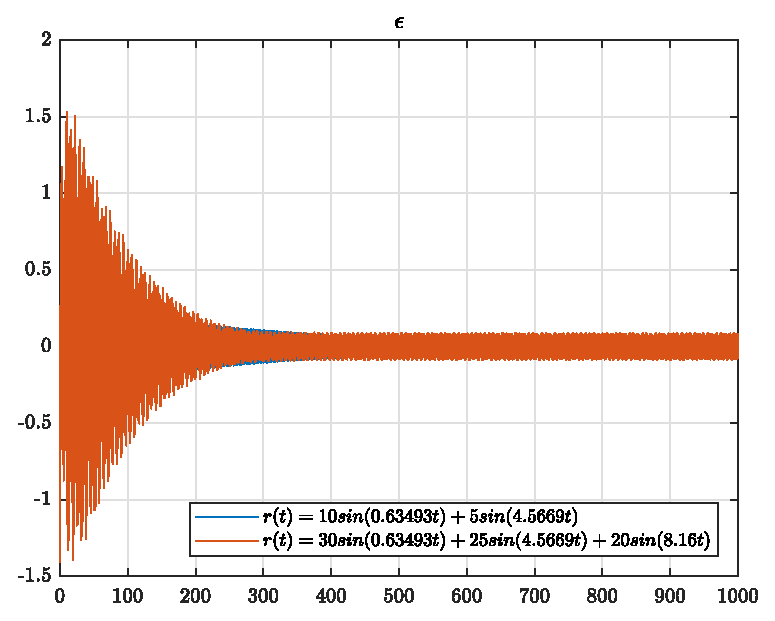
\includegraphics[width=12cm]{figs/gradiente/epsilon/sim03_r1r2.eps} 
\end{figure}
%---------------------------------------------------------------------